
\newpage 
\subsection*{Question 3a}
A four letter alphabet is encoded into binary form according to
\begin{center}
\begin{tabular}{|c|c|c|c|c|}
\hline Case 1	&	A:  10 	&	C:  110	&	G:  111 &	T:  0  \\ \hline
Case 2	&	A:  00	&	C:  01	&		G: 10	&	T: 11	\\ \hline
\end{tabular} 
\end{center}
Using the code presented in case 1, decode the following sequence:
\begin{verbatim}	
11110001011010
\end{verbatim}

\noindent Encode this message using the code from case 2. Compare the length of messages in both cases.

\subsection*{Question 3b}
Given that the alphabet has the following distribution 
\begin{center}
\begin{tabular}{|c|c|c|c|c|c|}
\hline
$x_i$	& A	& C	& G	& T \\ \hline
$p(x_i)$	& 0.25	& 0.125	& 0.125	& 0. 5 \\ \hline
\end{tabular} 
\end{center}
Compute the average symbol length for both cases.



%----------------------------------------------------------------------------- %
\section*{Question 3b}
\begin{center}
\begin{tabular}{|c|c|c|c|c|c|}
\hline 
	&	A	&	C	&	G	&	T	&		\\ \hline	
Code 1	&	10	&	110	&	111	&	0	&		\\ \hline	
$p(x_i)$	&	0.25	&	0.125	&	0.125	&	0.5	&		\\ \hline	
$n(x_i)$	&	2	&	3	&	3	&	1	&		\\ \hline	
$p(x_i) \times n(x_i)$	&	0.5	&	0.375	&	0.375	&	0.5	&	\textbf{1.75}	\\ \hline	
	&		&		&		&		&		\\ \hline	\hline
Code 2	&	00	&	01	&	10	&	11	&		\\ \hline	
$p(x_i)$	&	0.25	&	0.125	&	0.125	&	0.5	&		\\ \hline	
$n(x_i)$	&	2	&	2	&	2	&	2	&		\\ \hline	
$p(x_i) \times n(x_i)$	&	0.5	&	0.25	&	0.25	&	1	&	\textbf{2}	\\ \hline	
\end{tabular} 
\end{center}

Expected Code Lengths $E(L)$ for Codes 1 and 2 are 1.75b and 2b respectively.

%----------------------------------------------------------------------------- %
\section*{Question 5}
\begin{center}
\begin{tabular}{|c|c|c|c|c|c|c|c|}
\hline	&		&	Shannon Fano	&	Huffman	&		&		&		&	\\	
	&		&	 Code	&	Code	&	$n(x_i)$	&	$p(x_i) \times n(x_i)$	&	$I(x_i)$	&	$p(x_i) \times I(x_i)$	\\ \hline
$x_5$	&	0.50	&		&		&	1	&	0.50	&	1	&	0.5000	\\ \hline
$x_1$	&	0.20	&		&		&	2	&	0.40	&	2.3219	&	0.4644	\\ \hline
$x_2$	&	0.15	&		&		&	3	&	0.45	&	2.7370	&	0.4105	\\ \hline
$x_4$	&	0.10	&		&		&	4	&	0.40	&	3.3219	&	0.3322	\\ \hline
$x_3$	&	0.05	&		&		&	4	&	0.20	&	4.3219	&	0.2161	\\ \hline
	&		&		&		&		&	1.95	&		&	1.9232	\\ \hline
 
\end{tabular} 
\end{center}

\newpage 
%-----------------------------------------%
\subsection*{Question 4}
A DMS X has live symbols $\{x_l,x_2,x_3,x_4,x_5\}$ with $P(x_1) = 0.4$, $P(x_2)=0.19$, $P(x_3) =0.16$,
$P(x_4) = 0.15$, and $P(x_5) = 0.1$.
\begin{itemize}
\item[(a)] Construct the Shannon-Fano code for X, and calculate the efficiency of the code.
\item[(b)] Repeat for the Huffman code and compare the results.
\end{itemize}

\subsection*{Question 5}

A discrete memoryless source has a five symbol alphabet $\{x_1,x_2,x_3,x_4,x_5\}$ with the following probabilities 0.2,0.15,0.05,0.10 and 0.5.

\begin{itemize}
\item[(i)] Construct a Shannon-Fano code for $X$, and calculate the code efficiency.
\item[(ii)] Construct a Huffman code for $X$, and calculate the code efficiency.
\end{itemize}

%------------------------------------------------------------ %

%------------------------------------------------------------ %
\subsection*{Question 6}

The input source to a noisy communication channel is a random variable X over three symbols a,b,c. The output from this channel is a random variable Y over the same three symbols. The joint distribution of these two random variables is as follows:


\begin{center}
\begin{tabular}{|c|c|c|c|}
\hline	 &x=a	&x=b&	     x=c\\ \hline
y=a	 &0.25	&0	 &    0.125 \\ \hline
y=b	 &0	    &0.125&	 0 \\ \hline
y=c	 &0.125&	0.25&	 0.125 \\ \hline
\end{tabular} 
\end{center}

\begin{itemize}
\item Write down the marginal distributions for X and Y. %(Last Week)
\item Compute the marginal entropies $H(X)$ and $H(Y)$ %(Last Week)
\item Compute the joint entropy $H(X,Y)$ of the two random variables. % (Last Week)
\item
Compute the mutual information $I(X;Y)$.
\item 
Compute the conditional entropies $H(X|Y)$ and $H(Y|X)$.
\item 
From Formulae: \[I(X,Y) = H(X) — H(X|Y)\]
\end{itemize}
%------------------------------------------------------------ %
\subsection*{Question 7}

The frequency of 0 as an input to a binary channel is 0.6. If 0 is the input, then 0 is the output with probability 0.8. If l is the input, then l is the output with probability 0.9.

Write out the channel transition matrix

\begin{itemize}
\item	Calculate the output probabilities [P(Y)] 
\item	Compute the joint probabilities [P(X,Y)]
\item	Calculate the probability that the input is 0 given that the output is O. 
\item Calculate the probability that the input is l given that the output is 1, 
\item	Calculate the probability that the input is l given that the output is O.
\item	Calculate the probability that the input is 0 given that the output is l. 
\end{itemize}
%------------------------------------------------------------ %

%------------------------------------------------------------ %
%\section*{Question 4}

%-----------------------------------------%
\subsection*{Question 8 }
Consider a DMS X with symbols $\{x_l,x_2,x_3,x_4\}$. The table below lists four possible
binary codes.

\begin{figure}[h!]
\centering
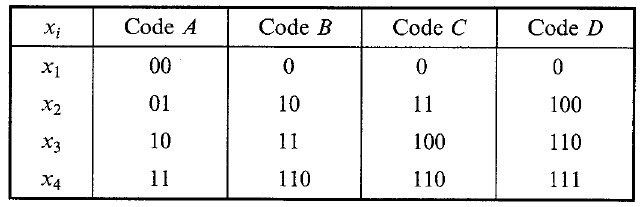
\includegraphics[width=0.7\linewidth]{./12ACodes}
\caption{}
\label{fig:12ACodes}
\end{figure}



%IMAGE OF KRAFT INEQUALITY HERE
\begin{itemize}
\item[(i)] Show that all codes except B satisfy the Kraft inequality (formula below)
m
\item[(ii)] Show that codesA and D are uniquely decodable but code B and C are not
uniquely demdable.
\end{itemize}
\begin{figure}[h!]
\centering
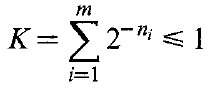
\includegraphics[width=0.4\linewidth]{./12AKraftIneq}
\caption{}
\label{fig:12AKraftIneq}
\end{figure}


%-----------------------------------------%
\subsection*{Question 9}
A DMS X has live symbols $\{x_l,x_2,x_3,x_4,x_5\}$ with $P(x_1) = 0.2$, $P(x_2)=0.15$, $P(x_3) =0.05$,
$P(x_4) = 0.10$, and $P(x_5) = 0.5$. 
\begin{itemize}
\item[(a)] Construct a Shann0n—Fano code for X, and calculate the efficiency of the code.
\item[(b)] Repeat for the Huffman code and compare the results.
\end{itemize}

 
\end{document}
\item
